% Source: graduate-coursework/Sp26/CSCE763/Course_Assignments/Project/project_proposal.tex
% Description: U-Net encoder-decoder architecture with skip connections for per-pixel radar target segmentation.

\documentclass[border=4pt]{standalone}
\usepackage{amsmath}
\usepackage{amssymb}
\usepackage{graphicx}
\usepackage{tikz}
\usepackage{xcolor}
\usetikzlibrary{positioning, arrows.meta, calc, fit, backgrounds, decorations.pathreplacing}

\definecolor{USC_Garnet}{HTML}{73000A}
\definecolor{USC_Black10}{HTML}{ECECEC}
\definecolor{USC_Black70}{HTML}{5C5C5C}
\definecolor{USC_Congaree}{HTML}{1F414D}

\begin{document}
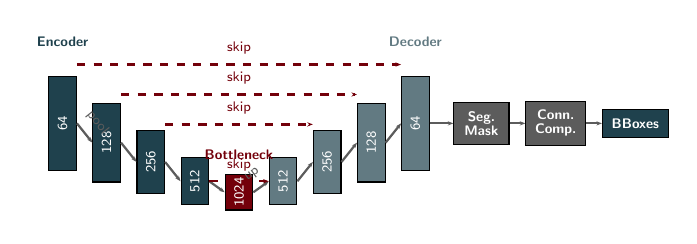
\begin{tikzpicture}[
  scale=0.7, every node/.style={font=\sffamily\tiny},
  enc/.style={draw, fill=USC_Congaree, text=white, minimum width=0.35cm,
    font=\sffamily\tiny\bfseries, align=center},
  dec/.style={draw, fill=USC_Congaree!70, text=white, minimum width=0.35cm,
    font=\sffamily\tiny\bfseries, align=center},
  nblock/.style={draw, fill=USC_Black70, text=white, minimum height=0.35cm,
    minimum width=0.7cm, font=\sffamily\tiny\bfseries, align=center},
  arr/.style={-{Stealth[length=2pt]}, thick, USC_Black70},
  skip/.style={-{Stealth[length=2pt]}, thick, USC_Garnet, dashed}
]
  % Encoder path (left side, going down)
  \node[enc, minimum height=1.2cm] (e1) at (0, 0) {};
  \node[enc, minimum height=1.0cm] (e2) at (0.8, -0.35) {};
  \node[enc, minimum height=0.8cm] (e3) at (1.6, -0.7) {};
  \node[enc, minimum height=0.6cm] (e4) at (2.4, -1.05) {};

  % Bottleneck
  \node[draw, fill=USC_Garnet, text=white, minimum height=0.45cm,
    minimum width=0.35cm, font=\sffamily\tiny\bfseries] (bn) at (3.2, -1.25) {};

  % Decoder path (right side, going up)
  \node[dec, minimum height=0.6cm] (d4) at (4.0, -1.05) {};
  \node[dec, minimum height=0.8cm] (d3) at (4.8, -0.7) {};
  \node[dec, minimum height=1.0cm] (d2) at (5.6, -0.35) {};
  \node[dec, minimum height=1.2cm] (d1) at (6.4, 0) {};

  % Labels on blocks
  \node[white, rotate=90, font=\sffamily\tiny] at (e1) {64};
  \node[white, rotate=90, font=\sffamily\tiny] at (e2) {128};
  \node[white, rotate=90, font=\sffamily\tiny] at (e3) {256};
  \node[white, rotate=90, font=\sffamily\tiny] at (e4) {512};
  \node[white, rotate=90, font=\sffamily\tiny] at (bn) {1024};
  \node[white, rotate=90, font=\sffamily\tiny] at (d4) {512};
  \node[white, rotate=90, font=\sffamily\tiny] at (d3) {256};
  \node[white, rotate=90, font=\sffamily\tiny] at (d2) {128};
  \node[white, rotate=90, font=\sffamily\tiny] at (d1) {64};

  % Encoder arrows (conv + pool, going down)
  \draw[arr] (e1.east) -- (e2.west) node[midway, above, sloped, font=\sffamily\tiny] {pool};
  \draw[arr] (e2.east) -- (e3.west);
  \draw[arr] (e3.east) -- (e4.west);
  \draw[arr] (e4.east) -- (bn.west);

  % Decoder arrows (upconv, going up)
  \draw[arr] (bn.east) -- (d4.west) node[midway, above, sloped, font=\sffamily\tiny] {up};
  \draw[arr] (d4.east) -- (d3.west);
  \draw[arr] (d3.east) -- (d2.west);
  \draw[arr] (d2.east) -- (d1.west);

  % Skip connections (horizontal dashed arrows)
  \draw[skip] (e4.east |- d4.west) -- (d4.west)
    node[midway, above, font=\sffamily\tiny, USC_Garnet] {skip};
  \draw[skip] ([yshift=0.1cm]e3.north east) -- ([yshift=0.1cm]d3.north west)
    node[midway, above, font=\sffamily\tiny, USC_Garnet] {skip};
  \draw[skip] ([yshift=0.15cm]e2.north east) -- ([yshift=0.15cm]d2.north west)
    node[midway, above, font=\sffamily\tiny, USC_Garnet] {skip};
  \draw[skip] ([yshift=0.2cm]e1.north east) -- ([yshift=0.2cm]d1.north west)
    node[midway, above, font=\sffamily\tiny, USC_Garnet] {skip};

  % Output: segmentation mask -> connected components -> bounding boxes
  \node[nblock, right=0.3cm of d1] (mask) {Seg.\\[-1pt]Mask};
  \node[nblock, right=0.2cm of mask] (cc) {Conn.\\[-1pt]Comp.};
  \node[draw, fill=USC_Congaree, text=white, minimum height=0.35cm,
    minimum width=0.7cm, font=\sffamily\tiny\bfseries, right=0.2cm of cc] (bbx) {BBoxes};

  \draw[arr] (d1.east) -- (mask.west);
  \draw[arr] (mask) -- (cc);
  \draw[arr] (cc) -- (bbx);

  % Section labels
  \node[USC_Congaree, font=\sffamily\tiny\bfseries, anchor=south] at ([yshift=0.35cm]e1.north) {Encoder};
  \node[USC_Garnet, font=\sffamily\tiny\bfseries, anchor=south] at ([yshift=0.08cm]bn.north) {Bottleneck};
  \node[USC_Congaree!70, font=\sffamily\tiny\bfseries, anchor=south] at ([yshift=0.35cm]d1.north) {Decoder};
\end{tikzpicture}
\end{document}
